\documentclass{article}
\usepackage{iclr2026_conference,times}

\input{math_commands.tex}

\usepackage{amsmath,amssymb,amsthm}
\usepackage{booktabs}
\usepackage{graphicx}
\usepackage{hyperref}
\usepackage{url}

\title{A Regression Theory of Dissociation Between Brain Prediction and Control}

% Keep anonymous for ICLR submission.
\author{Anonymous Authors}

\newtheorem{proposition}{Proposition}
\newcommand{\bbeta}{\boldsymbol{\beta}}
\newcommand{\bhat}{\widehat{\boldsymbol{\beta}}}
\newcommand{\btrue}{\boldsymbol{\beta}^{\star}}
\newcommand{\x}{\mathbf{x}}
\newcommand{\uhat}{\mathbf{u}}
\newcommand{\df}{\mathrm{df}_{2}}
\newcommand{\Eacc}{E_{\mathrm{acc}}}

%\iclrfinalcopy
\begin{document}
\maketitle

\begin{abstract}
Deep neural network encoding models can accurately predict visual neuronal responses to natural images, yet their success in generating images that control neuronal activity varies dramatically. Recent systematic evaluations reveal three linked observations: strong prediction does not ensure controllability; poor controllers often produce high-spatial-frequency modulations that are ineffective for neurons; and some poor controllers can still predict which stimuli generated by better controllers will succeed. We develop a regression theory for this prediction-control dissociation. Prediction depends on the inner product $\mathbf{w}^{\top}\mathbf{x}$ between model weights and natural-image features, whereas control by feature accentuation follows the weight direction $\mathbf{w}$ itself. Because natural images have highly anisotropic covariance, low-variance high-frequency directions can be weakly constrained by prediction but strongly amplified during control. In a linear regression model, learned weights can acquire substantial off-manifold components with little effect on held-out prediction, producing ineffective accentuation images while still evaluating on-manifold controls generated by better-aligned models. We then apply random matrix theory to predict how sample size, feature dimensionality, regularization, and neuronal noise determine which weight modes are error-prone. The theory decomposes coefficient error into regularization bias, finite-sample signal fluctuation, and noise amplification, and is validated against ordinary least squares, ridge, and sparse regression simulations on natural-image spectra. Together, the framework explains why good encoders can be poor controllers and motivates on-manifold feature accentuation for robust closed-loop neural control.
\end{abstract}

\section{Introduction}

Deep encoding models are increasingly used not only to predict neural responses, but also to synthesize stimuli for neural control. The workflow is conceptually simple: fit a model $f$ to neural responses on natural images, then optimize an image so that $f$ predicts a target response. If the model is a reliable surrogate for the neuron, this procedure should generate effective control stimuli.

The empirical picture is more puzzling. Models with similar held-out encoding accuracy can generate very different accentuated images and achieve very different control levels. In the visual encoding experiments motivating this work, a standard ResNet50 encoder and a robust ResNet50 encoder can both predict responses to natural images, but their accentuation images differ qualitatively: one produces high-frequency, visually unnatural modulations, while the other produces lower-frequency, more semantic image changes. More surprisingly, a model that fails as a controller can still act as a useful evaluator: it can predict that stimuli generated by another, better-aligned model will drive the neuron, even though optimizing its own gradient produces ineffective images.

This pattern suggests a specific failure mode. Prediction tests model outputs on the natural-image distribution. Control follows model gradients. These are not equivalent. A model can have the right input-output relation on natural images while having a gradient direction that points away from the natural-image manifold.

We study this dissociation in a simplified linear setting. The central contrast is that prediction evaluates a scalar response on natural images, whereas control follows the model's weight or gradient direction. If natural images have many low-variance directions, large errors in those directions can be nearly invisible to held-out prediction but dominate the synthesized control image. This paper develops a theory of that empirical puzzle and uses RMT to identify which modes are most error-prone.

Our contributions are:
\begin{itemize}
    \item We formalize a prediction-control dissociation motivated by visual neural control: matching prediction on natural images can hide weight differences that are exposed by feature accentuation.
    \item We show that a linear toy model reproduces the empirical asymmetry: a bad controller can still predict the success of stimuli generated by a better controller.
    \item We apply random matrix theory (RMT) to derive a three-term deterministic equivalent for per-eigenmode regression error under anisotropic natural-image covariance.
    \item We use the formula to predict when low-variance modes become unstable, when accentuation error diverges from ordinary generalization error, and how the failure depends on $n$, $d$, $\lambda$, and noise level.
    \item We diagnose a second-order alignment-variance gap and give a delta-method correction showing why leading deterministic equivalents accurately predict $\mathbb{E}[R]$ but can underpredict $\mathbb{E}[(1-R)^2]$ in high-noise regimes.
\end{itemize}

\section{Related Work}

\paragraph{High-dimensional regression and RMT.}
High-dimensional linear regression has been a central testbed for understanding bias, variance, interpolation, and regularization in modern machine learning \citep{dobriban2018high,hastie2022surprises,mei2022generalization}. Deterministic equivalents from random matrix theory provide sharp asymptotic predictions for ridge risk under anisotropic covariance and proportional scaling \citep{bai2010spectral,couillet2011random}. Our work uses this toolbox but shifts the target from scalar predictive risk to a directional error induced by using the learned coefficient vector as an intervention axis.

\paragraph{Feature visualization and neural control.}
The problem is also related to representation analysis, feature visualization, and feature accentuation, where gradients are used to generate or modify images that drive model units \citep{olah2017feature,bau2017network,hamblin2024feature}. In neural control, these methods are used not only to interpret a model but also to synthesize candidate stimuli for biological validation. In such settings, average predictive accuracy is not sufficient: one needs the learned direction to be geometrically aligned with the intended neural factor. The accentuation metric studied here is a minimal linear analogue of this directional reliability problem.

\section{Empirical Puzzle: Prediction Is Not Control}

The motivating experiments compare encoding models trained to predict visual neuronal responses from natural images and then used for model-based control by feature accentuation. The core observations are:
\begin{enumerate}
    \item \textbf{Matched prediction.} Different encoders can have similar train and test prediction accuracy on natural images.
    \item \textbf{Divergent control.} The same encoders can generate very different accentuation images and achieve very different neural control levels. Poor controllers often produce high-spatial-frequency changes.
    \item \textbf{Prediction-control asymmetry.} A model that fails to generate effective control stimuli can still predict that stimuli generated by a better controller will be effective.
\end{enumerate}

\begin{figure}[p]
    \centering
    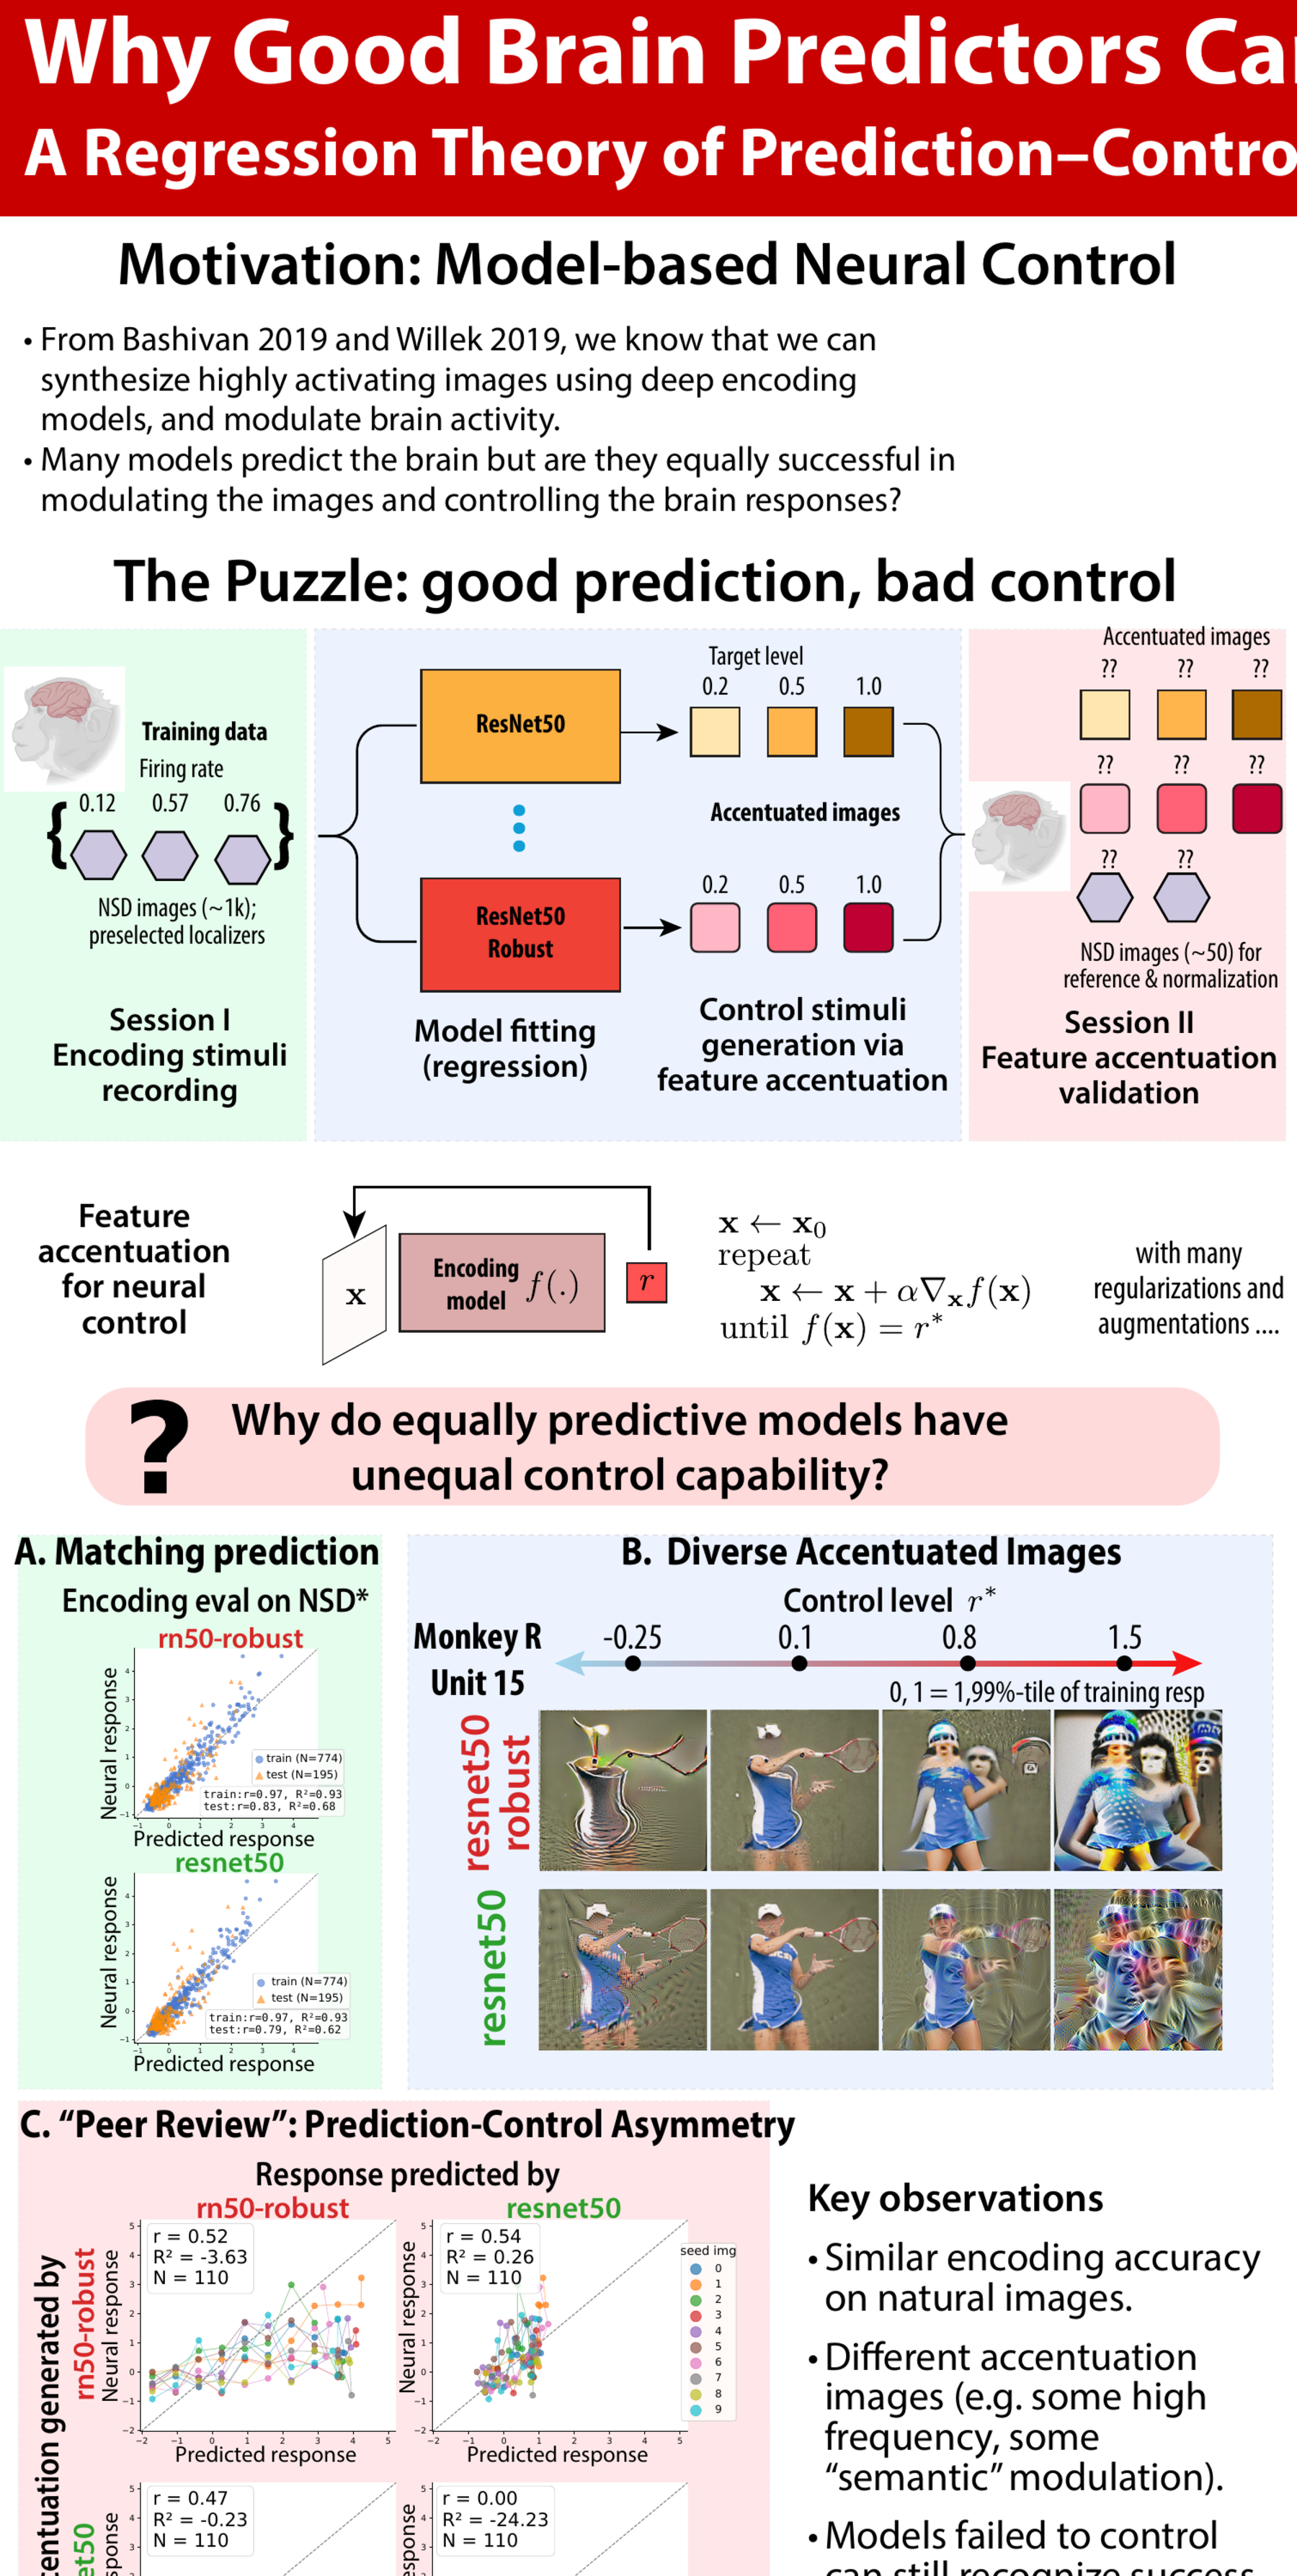
\includegraphics[height=.74\textheight,keepaspectratio]{../figures/empirical_prediction_control_puzzle.png}
    \caption{Empirical motivation. Deep encoding models can have similar prediction accuracy on natural images but produce different feature-accentuated control images. The motivating experiments show three observations: matched encoding accuracy, divergent control images and control levels, and a prediction-control asymmetry in which a poor generator can still recognize effective stimuli generated by another model.}
    \label{fig:empirical_puzzle}
\end{figure}

These observations point to a geometry mismatch. Encoding evaluation samples images from $p(\x)$ and measures outputs $f(\x)$. Control differentiates the model and follows $\nabla_\x f$. For a linear model $f(\x)=\mathbf{w}^{\top}\x$, this distinction is exact: prediction depends on the weight-input product, but control follows the weight vector itself. Two weights can therefore agree on natural images if their difference lies in low-variance directions of $p(\x)$, while producing radically different gradients.

Natural images make this problem severe. Their covariance spectrum is highly anisotropic: high-frequency components often correspond to low-variance principal components. Therefore, noise or finite-sample fluctuations can create large coefficients in high-frequency directions with little penalty under natural-image prediction. During gradient-based synthesis, those coefficients are no longer suppressed by the image distribution and can dominate the image update.

\section{A Linear Model Recreates the Puzzle}

The empirical observations can be recreated without deep networks. Consider a ground-truth neuron $f^\star(\x)={\btrue}^{\top}\x$ and two models $f_1(\x)=\mathbf{w}_1^\top\x$, $f_2(\x)=\mathbf{w}_2^\top\x$. Let $\mathbf{w}_1$ be close to $\btrue$ plus moderate perturbations in mid-variance directions, and let $\mathbf{w}_2$ include a much larger perturbation in bottom-eigenvalue directions of the natural-image covariance. On held-out natural images, both models can have nearly perfect prediction because the perturbation in $\mathbf{w}_2$ is almost orthogonal to the data distribution. But accentuation reveals the difference:
\begin{equation}
    \x_{\mathrm{acc},j}
    =
    \x_0+\frac{r^\star-\mathbf{w}_j^\top\x_0}{\|\mathbf{w}_j\|^2}\mathbf{w}_j .
\end{equation}
For $j=2$, the generated image moves along hidden low-variance directions and becomes high-frequency or off-manifold; for $j=1$, the generated image stays more aligned with the true neuronal axis.

The same setup explains the peer-review asymmetry. A model whose own accentuation path is poor can still evaluate another model's stimuli if those stimuli lie near the true axis or natural-image manifold. In notation, $f_2(\x_{\mathrm{acc},1})$ can correlate well with $f^\star(\x_{\mathrm{acc},1})$, even while $f^\star(\x_{\mathrm{acc},2})$ is poor. Evaluation asks whether the model's scalar output is correct on a particular stimulus set; generation asks whether its gradient points in a useful direction.

\section{Formal Setup}

We model the neuron and its encoding model as linear functions of image features. Training data follow
\begin{equation}
    y = {\btrue}^{\top} \x + \sigma \epsilon,
    \qquad \x\sim\mathcal{N}(0,\Sigma),
    \label{eq:linear_model}
\end{equation}
and the ridge estimator is
\begin{equation}
    \bhat = (X^\top X + n\lambda I)^{-1}X^\top y.
    \label{eq:ridge_estimator}
\end{equation}
Prediction on natural images depends on $\bhat^\top\x$. Therefore, if $\Sigma$ has many low-variance directions, large weight errors in those directions can have little effect on held-out prediction. By contrast, feature accentuation follows the weight itself:
\begin{equation}
    \x_{\mathrm{acc}} \leftarrow \x_0 + \alpha \bhat
    \quad\text{or}\quad
    \x_{\mathrm{acc}} = \x_0 + \frac{r^\star-\bhat^\top\x_0}{\|\bhat\|^2}\bhat .
    \label{eq:accentuation_path}
\end{equation}
The usual generalization error is
\begin{equation}
    E_{\mathrm{gen}} =
    \mathbb{E}_{X,\epsilon,\x}\bigl[(\bhat-\btrue)^\top \x\bigr]^2
    =
    \mathbb{E}_{X,\epsilon}(\bhat-\btrue)^\top\Sigma(\bhat-\btrue).
    \label{eq:gen_error}
\end{equation}
The corresponding accentuation error asks what happens when the fitted direction is used as the control path. If the target response is defined by $\btrue$ but the generated image moves along $\bhat$, the error is controlled by
\begin{equation}
    R=\frac{\bhat^\top\btrue}{\bhat^\top\bhat},
    \qquad
    \Eacc = {\btrue}^{\top}\Sigma\btrue \cdot \mathbb{E}\left[(1-R)^2\right].
    \label{eq:acc_error}
\end{equation}
This quantity is not a reweighted version of $E_{\mathrm{gen}}$: it is sensitive to the direction and norm of $\bhat$, and it can be dominated by modes that contribute little to average test error.

\section{RMT Explanation of Error-Prone Modes}

Let $\Sigma=\sum_{k=1}^{d}\lambda_k \uhat_k\uhat_k^\top$ and write $b_k=\uhat_k^\top\btrue$. Define $\kappa=\kappa(\lambda)$ as the positive solution of the fixed-point equation
\begin{equation}
    \kappa-\lambda
    = \gamma\kappa \frac{1}{d}\sum_{j=1}^{d}\frac{\lambda_j}{\kappa+\lambda_j}.
    \label{eq:kappa}
\end{equation}
We also define
\begin{equation}
    \df(\kappa)=\sum_{j=1}^{d}\frac{\lambda_j^2}{(\lambda_j+\kappa)^2},
    \qquad
    C_{\mathrm{sig}}(\kappa)=\sum_{j=1}^{d}\frac{\lambda_j b_j^2}{(\lambda_j+\kappa)^2}.
\end{equation}

\begin{proposition}[Per-eigenmode ridge error]
Under the Gaussian design model above and in the proportional high-dimensional limit, the squared coefficient error along the $k$th population eigenvector satisfies the deterministic equivalent
\begin{align}
    \mathbb{E}\bigl[(\uhat_k^\top(\bhat-\btrue))^2\bigr]
    &\asymp
    \underbrace{\frac{\kappa^2}{(\lambda_k+\kappa)^2}b_k^2}_{\text{regularization bias}}
    +
    \underbrace{
    \frac{1}{n-\df(\kappa)}
    \frac{\lambda_k\kappa^2}{(\lambda_k+\kappa)^2}
    C_{\mathrm{sig}}(\kappa)}_{\text{finite-sample signal fluctuation}}
    \nonumber\\
    &\quad+
    \underbrace{
    \frac{\sigma^2}{n-\df(\kappa)}
    \frac{\lambda_k}{(\lambda_k+\kappa)^2}}_{\text{finite-sample noise amplification}} .
    \label{eq:per_pc}
\end{align}
\end{proposition}

The three terms in equation~\ref{eq:per_pc} have distinct geometric meanings. The first term is deterministic shrinkage of true signal along eigenmodes of $\Sigma$. The second is a finite-sample fluctuation of the signal component induced by the random training design. The third is noise amplification; it peaks around $\lambda_k\approx\kappa$ and grows as $\kappa$ becomes small. Ordinary test error is obtained by summing equation~\ref{eq:per_pc} with weights $\lambda_k$:
\begin{equation}
    E_{\mathrm{gen}}\asymp
    \sum_{k=1}^{d}\lambda_k\,
    \mathbb{E}\bigl[(\uhat_k^\top(\bhat-\btrue))^2\bigr].
\end{equation}

\section{Accentuation Error}

The accentuation metric depends on the ratio
\begin{equation}
    R=\frac{\bhat^\top\btrue}{\bhat^\top\bhat}.
\end{equation}
Using equation~\ref{eq:per_pc}, the deterministic equivalents for numerator and denominator are
\begin{align}
    N_{\det}
    &= \sum_{k=1}^{d}\frac{\lambda_k}{\lambda_k+\kappa}b_k^2,\\
    D_{\det}
    &= \sum_{k=1}^{d}\left(\frac{\lambda_k}{\lambda_k+\kappa}\right)^2b_k^2
    +
    \frac{\kappa^2 C_{\mathrm{sig}}+\sigma^2}{n-\df(\kappa)}
    \sum_{k=1}^{d}\frac{\lambda_k}{(\lambda_k+\kappa)^2}.
\end{align}
Thus $R_{\det}=N_{\det}/D_{\det}$, and the leading accentuation prediction is
\begin{equation}
    \Eacc^{(0)}
    =
    {\btrue}^{\top}\Sigma\btrue\,(1-R_{\det})^2.
    \label{eq:eacc0}
\end{equation}

Equation~\ref{eq:eacc0} makes the dissociation from ordinary generalization explicit. $E_{\mathrm{gen}}$ weights per-mode error by the data variance $\lambda_k$, while accentuation depends on the ratio of two global quadratic forms in $\bhat$. As a result, the same ridge penalty can reduce average prediction error while producing a fitted direction whose extrapolation scale is biased.

\section{Regression and RMT Validation}

We evaluate two claims. First, anisotropic natural-image covariance makes prediction blind to some weight differences that are exposed by accentuation. Second, the RMT formula predicts which modes become unstable as sample size, dimensionality, regularization, and response noise change.

For the toy prediction-control experiments, we use van Hateren image patches as the natural-image distribution and define linear neurons with known pixel-space weights. We compare ordinary least squares, ridge regression, and sparse regression fits. Even when prediction error on held-out natural images remains small, subtle response noise can create visible high-frequency components in the learned weights. Ridge regularization prevents literal blow-up, but equation~\ref{eq:per_pc} predicts that modes near $\lambda_k\approx\kappa$ remain strongly amplified. These hidden components produce adversarial-looking feature accentuations while having minimal impact on natural-image prediction.

For the RMT checks, we evaluate the deterministic equivalents on three spectra: isotropic covariance, power-law covariance, and empirical covariance from van Hateren natural-image patches. Monte Carlo estimates are computed by repeatedly sampling $X$ and response noise, fitting ridge regression, and comparing the fitted coefficient vector to the ground-truth coefficient vector. For large dimensions we use the kernel form of ridge regression and GPU Monte Carlo.

\begin{figure}[t]
    \centering
    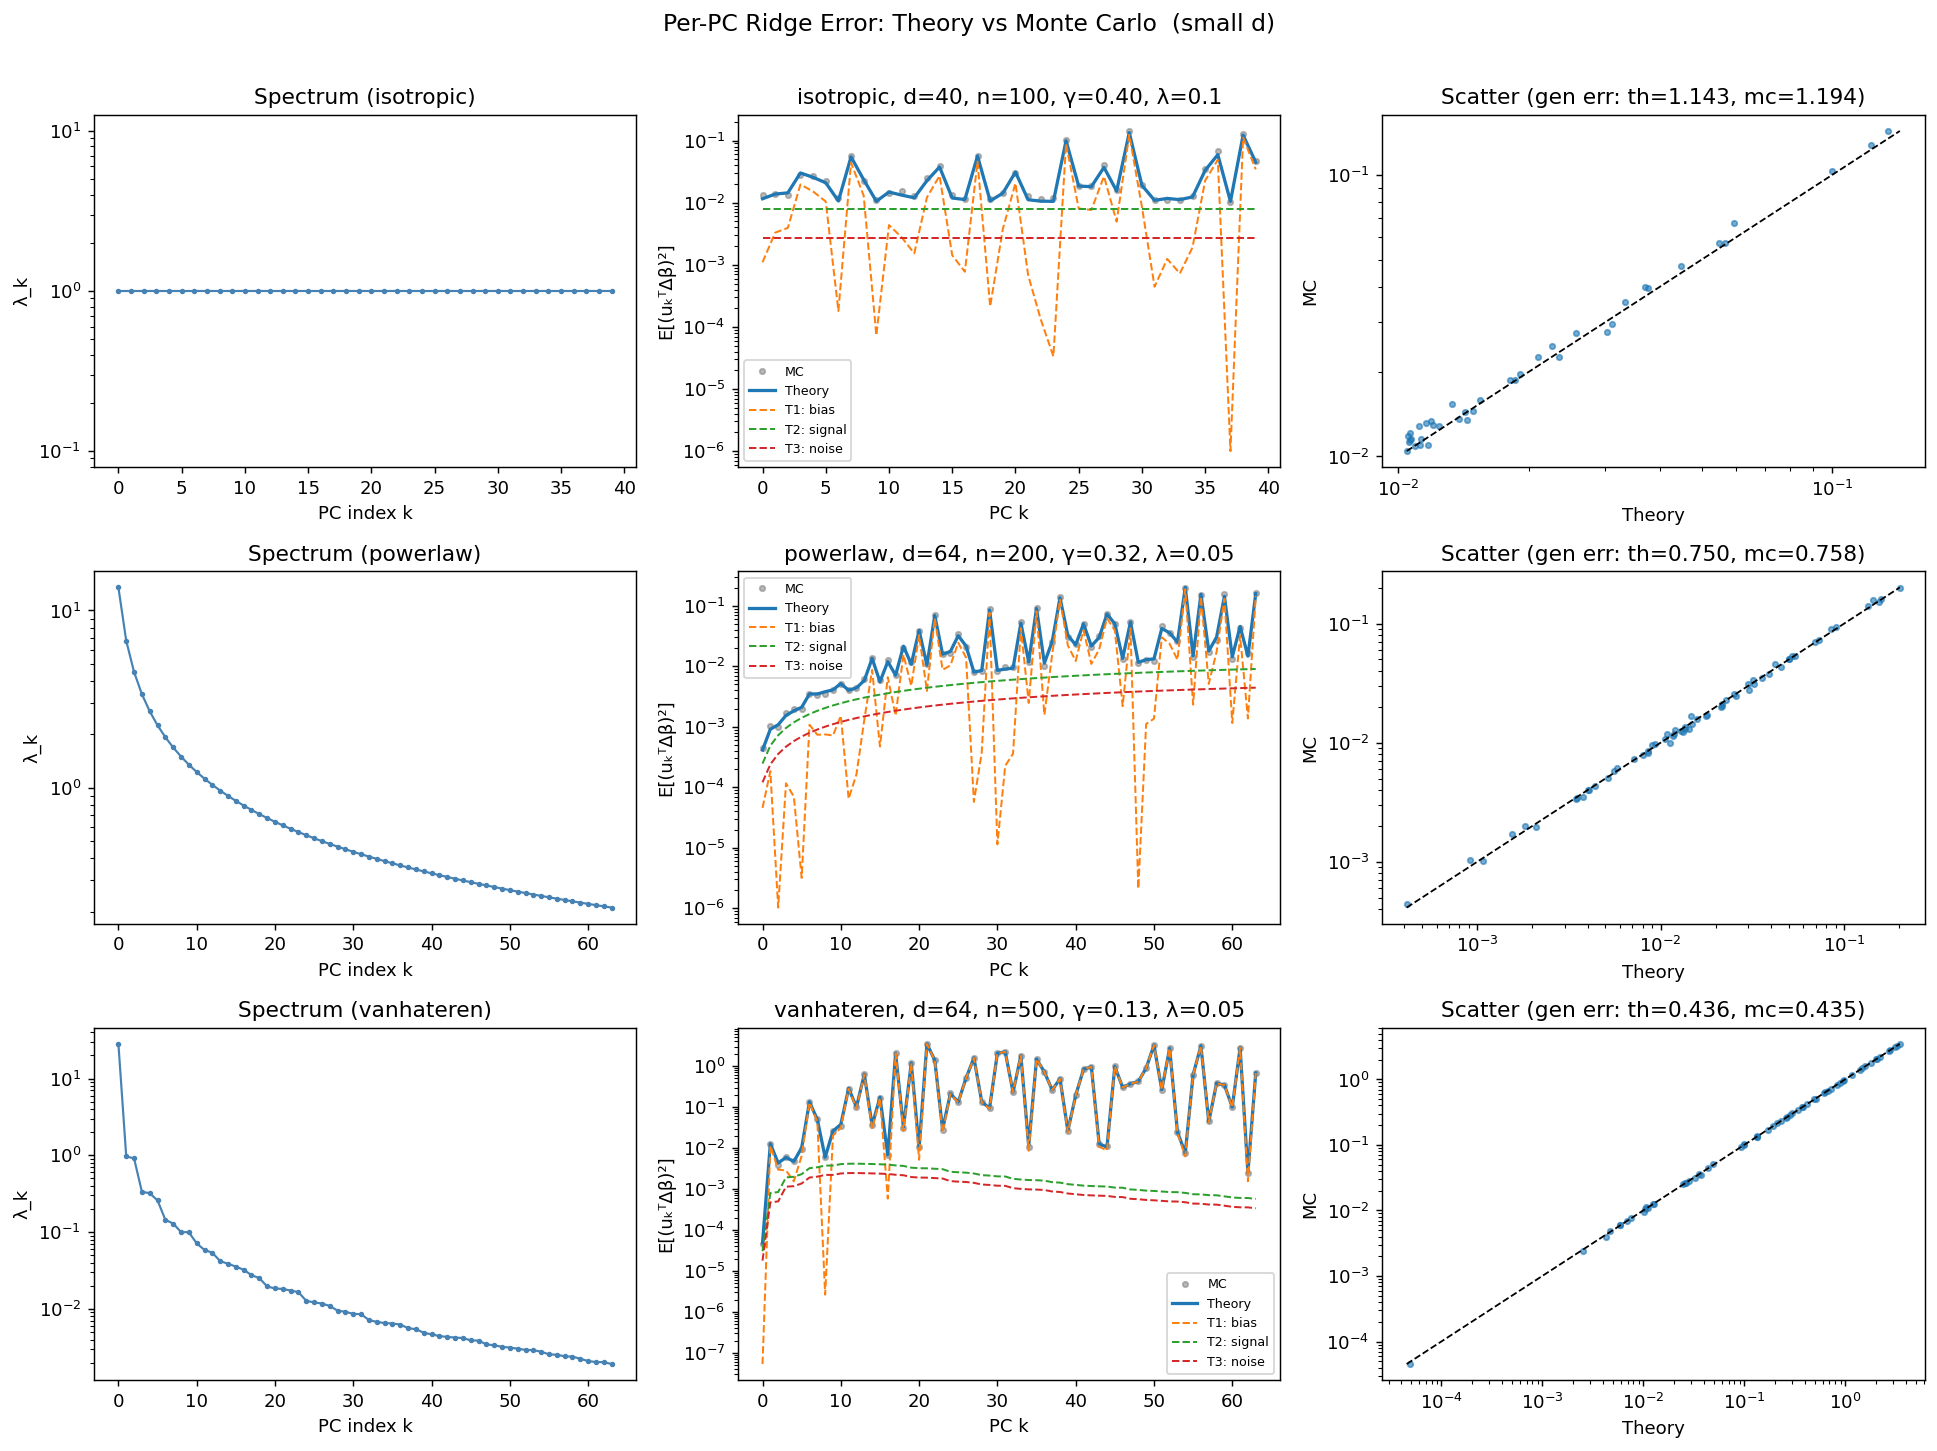
\includegraphics[width=\textwidth]{../figures/nb_small_d_per_pc.png}
    \caption{Per-eigenmode coefficient error. The three-term deterministic equivalent tracks Monte Carlo estimates across isotropic, power-law, and natural-image spectra, including the shape of the error across population PCs.}
    \label{fig:per_pc}
\end{figure}

Figure~\ref{fig:per_pc} validates equation~\ref{eq:per_pc} at small dimension, where per-PC Monte Carlo estimates are directly observable. The theory captures not only total error but also the anisotropic distribution of coefficient error across eigendirections.

\begin{figure}[t]
    \centering
    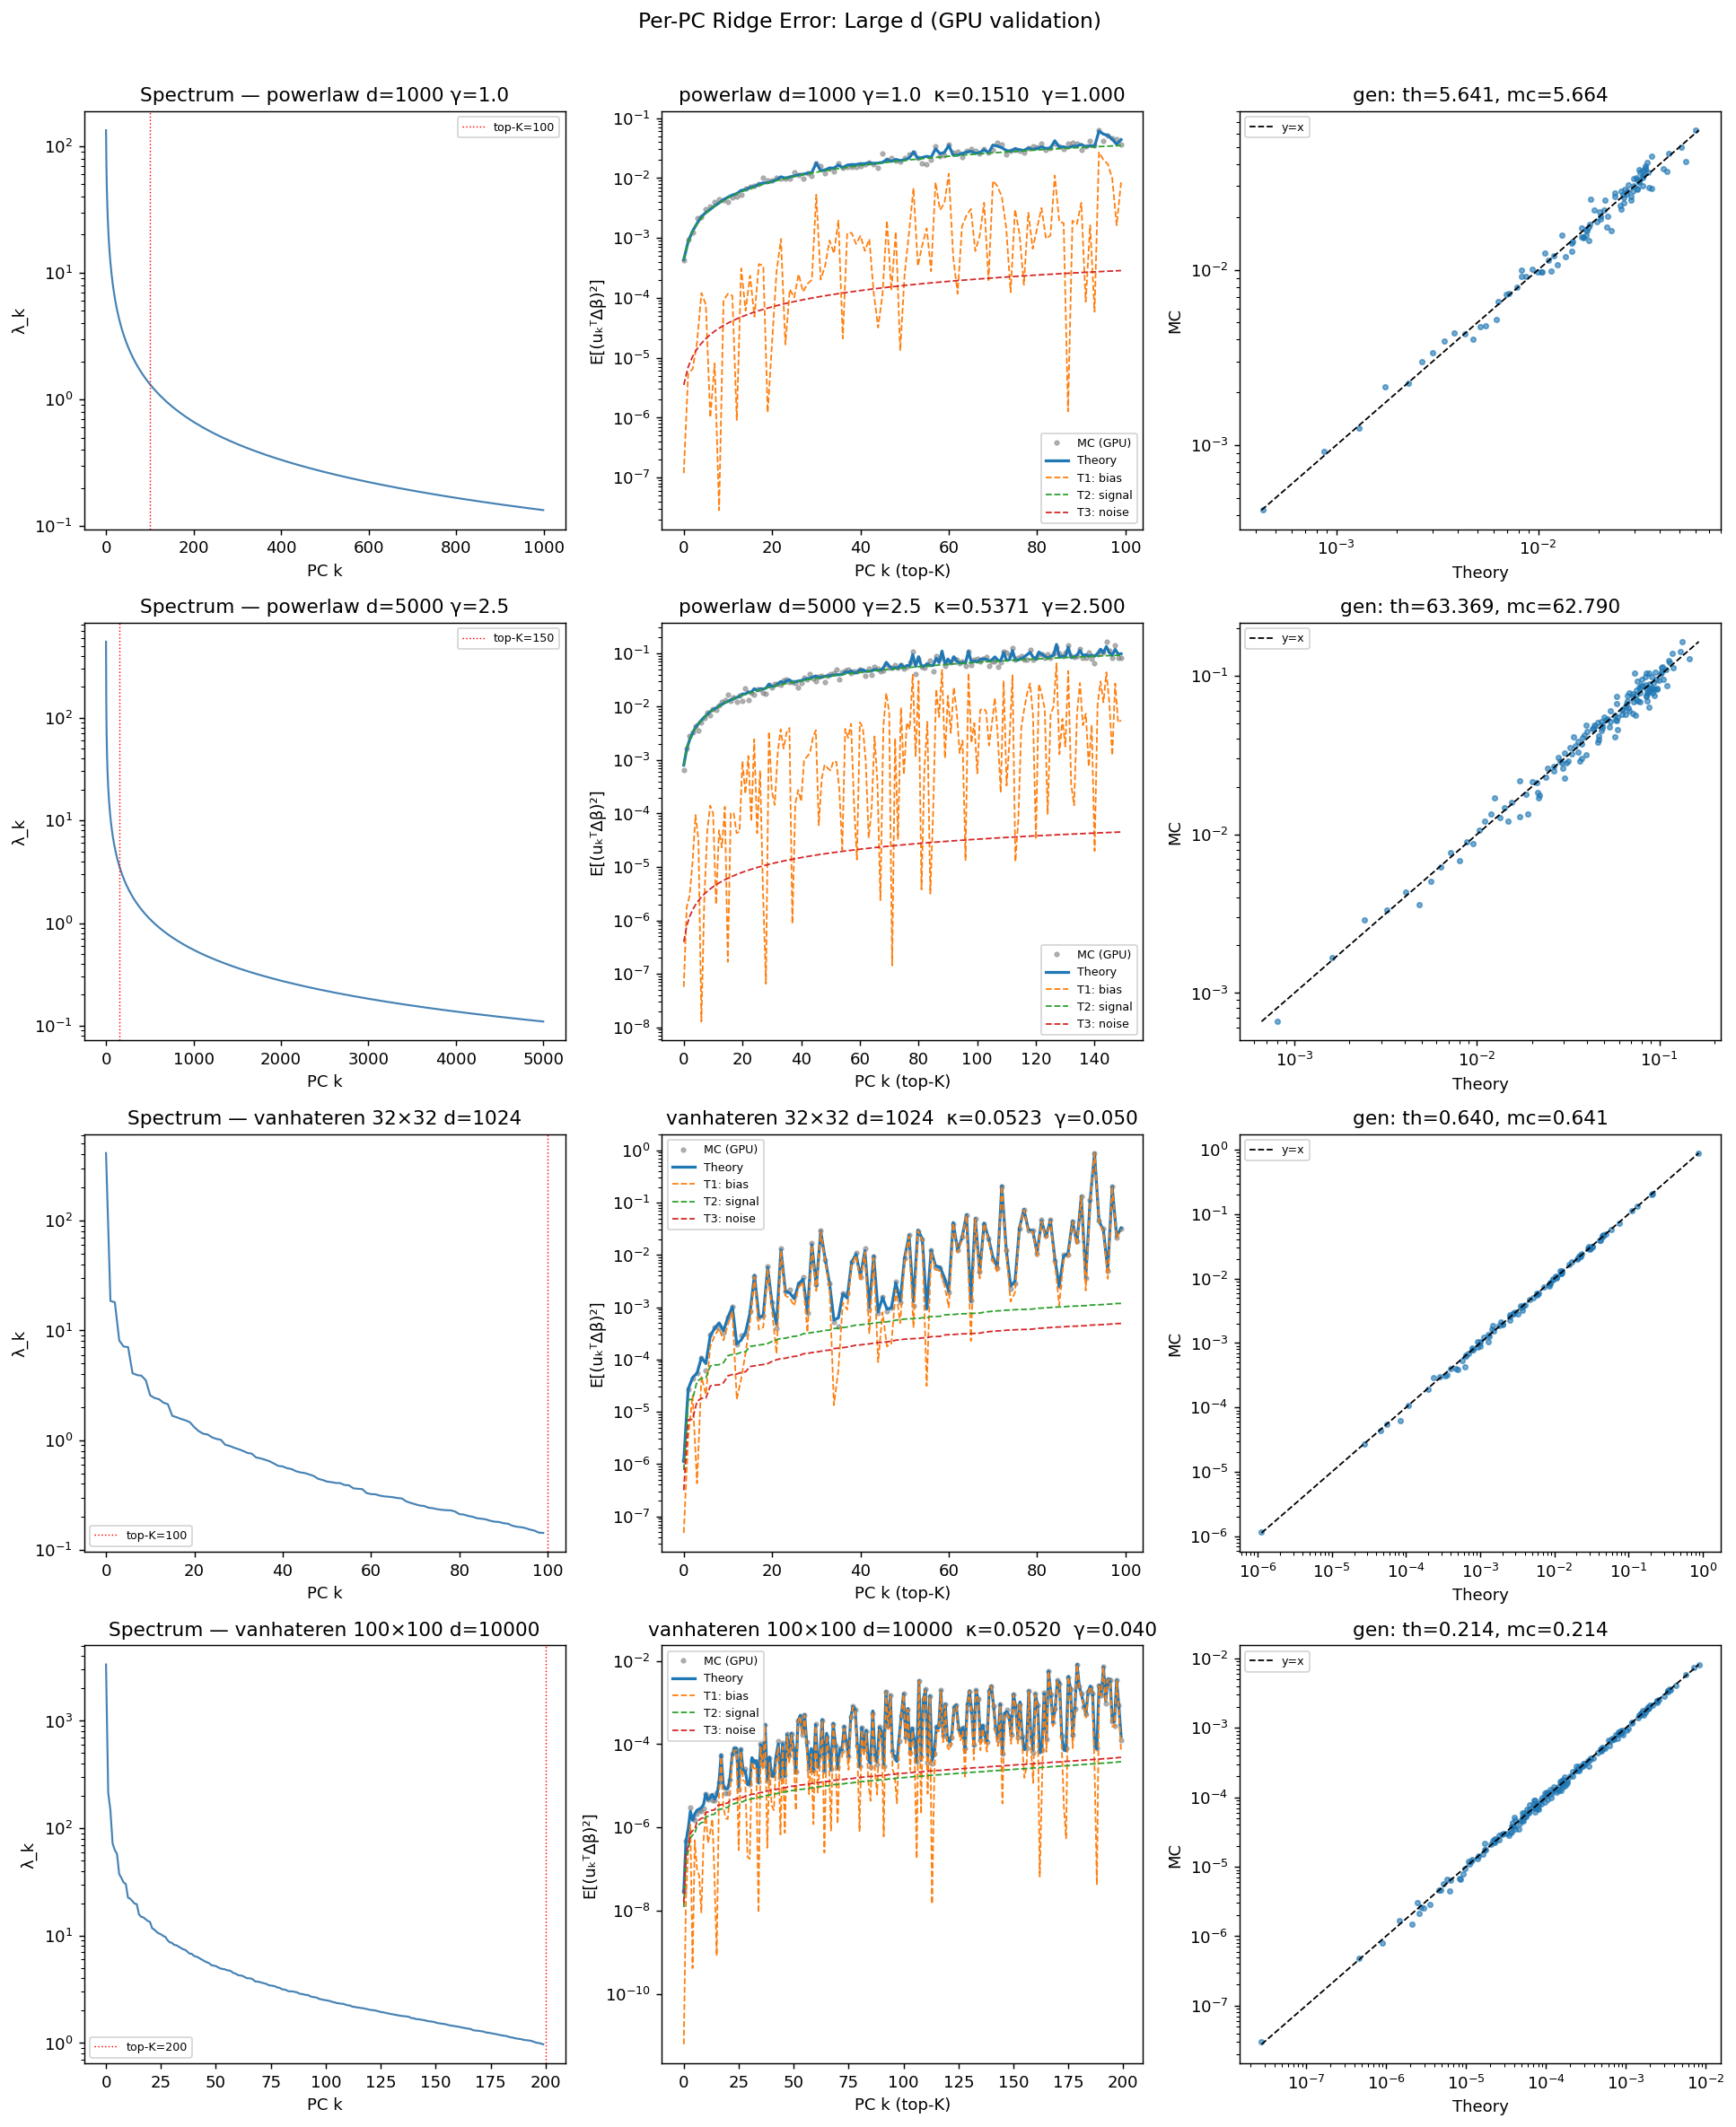
\includegraphics[width=\textwidth]{../figures/nb_large_d.png}
    \caption{Large-dimensional validation. GPU simulations agree with the deterministic equivalent for power-law spectra and natural-image covariance spectra up to $d=10{,}000$.}
    \label{fig:large_d}
\end{figure}

Figure~\ref{fig:large_d} confirms that the formulas remain accurate in the high-dimensional regime where the asymptotic theory is intended to apply. On power-law and natural-image spectra, total generalization error agrees with Monte Carlo to within the small gaps reported in the validation code.

\begin{figure}[t]
    \centering
    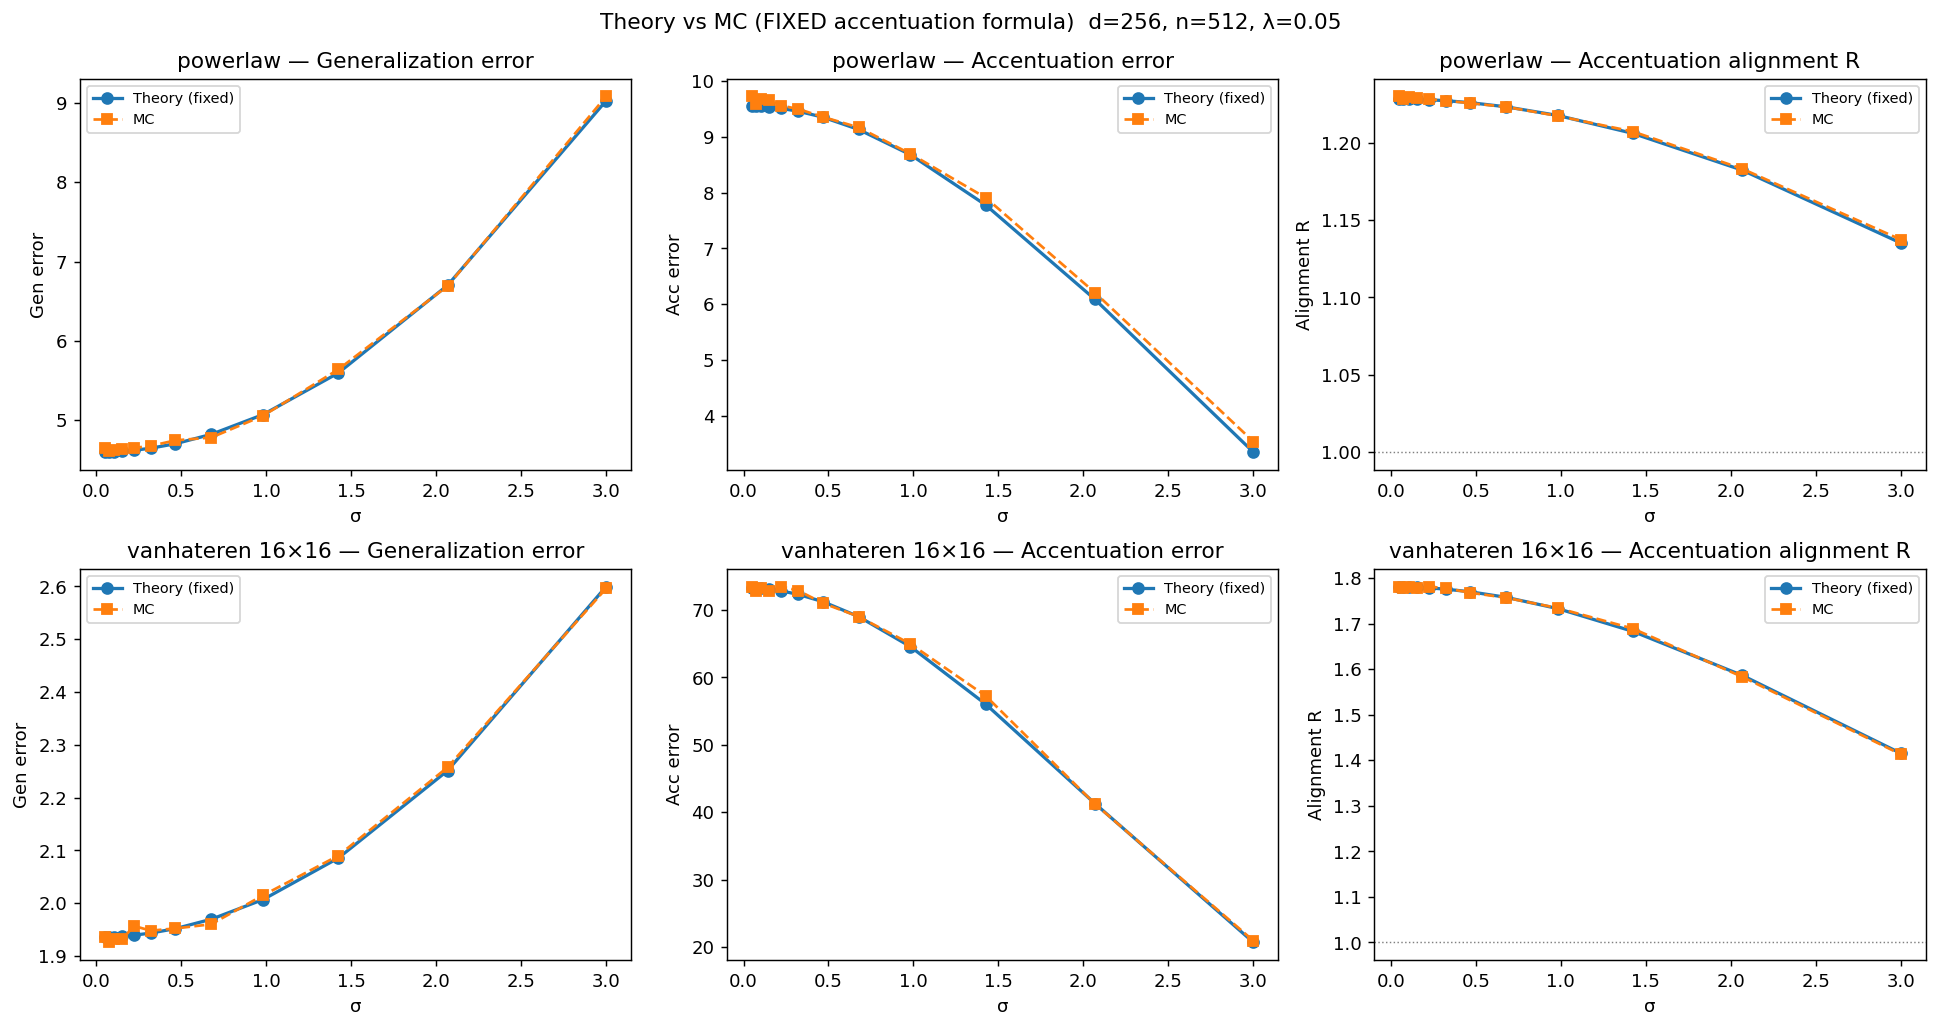
\includegraphics[width=\textwidth]{../figures/sigma_sweep_fixed_accentuation.png}
    \caption{Noise sweep. The deterministic equivalent tracks ordinary generalization error and the mean accentuation alignment across noise levels. Correctly accounting for finite-sample signal variance in $D_{\det}$ is essential for the alignment prediction.}
    \label{fig:sigma}
\end{figure}

Figure~\ref{fig:sigma} shows a sweep over response noise. The leading RMT prediction matches average generalization error across the full range, and it accurately predicts the mean alignment ratio $R$. This experiment also identifies a practical failure mode in incomplete formulas: replacing $\mathbb{E}[\bhat^\top\bhat]$ by a squared mean omits the finite-sample signal term and produces a biased alignment estimate.

\begin{figure}[t]
    \centering
    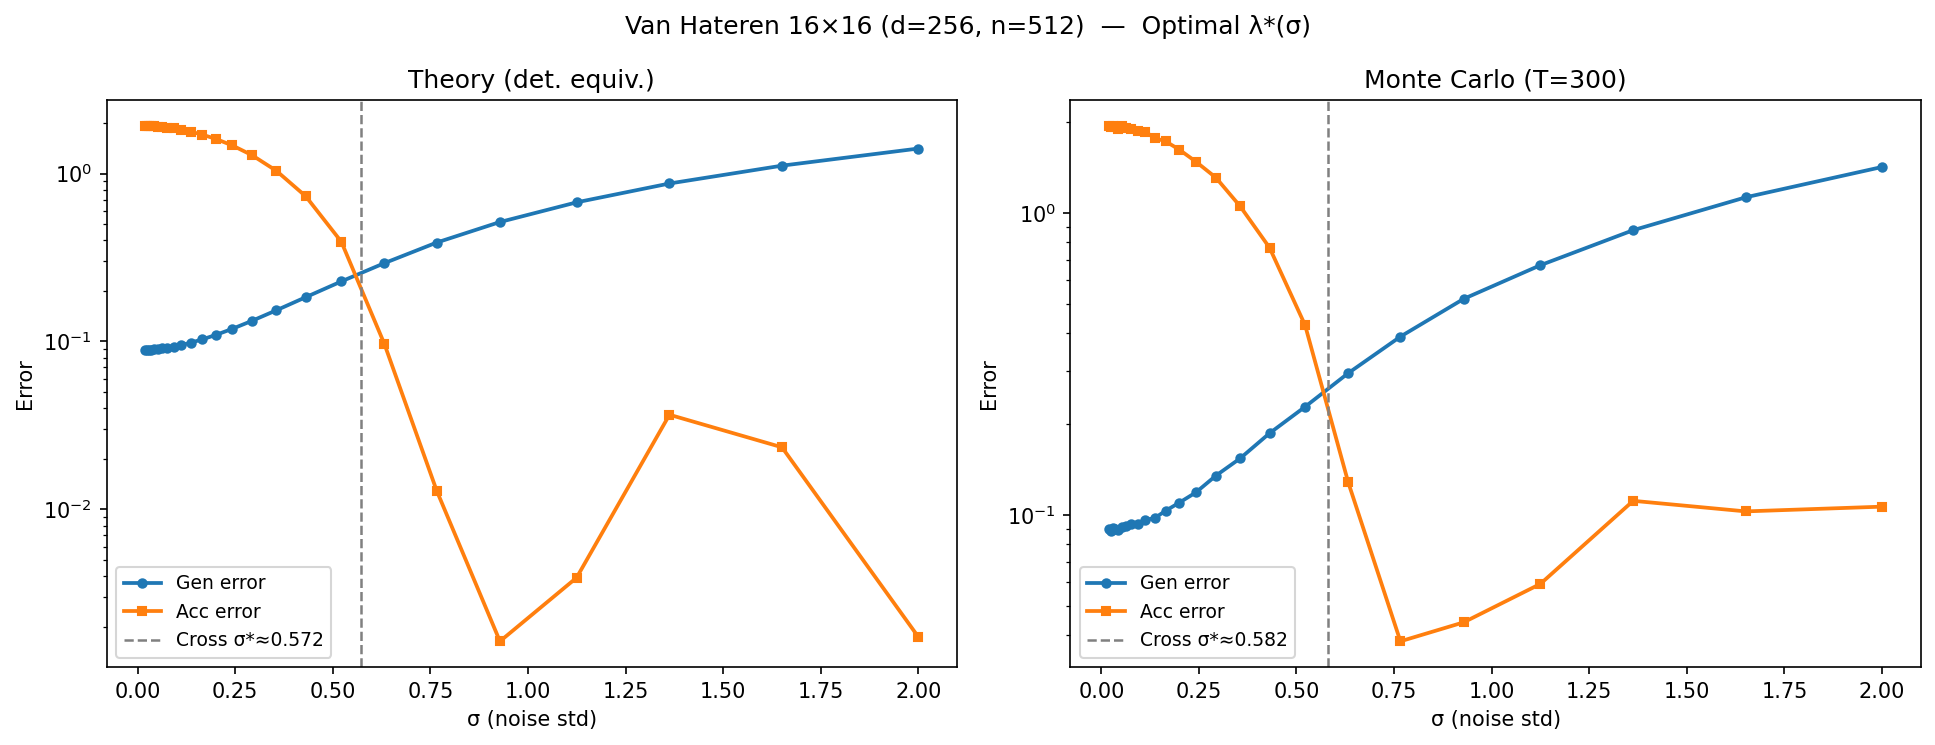
\includegraphics[width=.82\textwidth]{../figures/gen_vs_acc_optimal_lambda_vh.png}
    \caption{Generalization--accentuation crossing on van Hateren spectra. With $\lambda$ chosen to minimize predicted generalization error at each $\sigma$, the theory predicts the noise level at which ordinary test error overtakes accentuation error.}
    \label{fig:crossing}
\end{figure}

Figure~\ref{fig:crossing} illustrates the central qualitative prediction. At low noise, directional accentuation error can dominate because regularization biases the learned direction. At high noise, ordinary prediction error dominates because noise contaminates the coefficient estimate. The crossing point gives a concise operating-regime summary.

\section{Second-Order Gap: Variance of the Alignment Ratio}

The leading accentuation formula uses
\begin{equation}
    \mathbb{E}[(1-R)^2]\approx (1-R_{\det})^2.
\end{equation}
This is accurate when the bias term dominates. However,
\begin{equation}
    \mathbb{E}[(1-R)^2]=(1-\mathbb{E}R)^2+\operatorname{Var}(R),
\end{equation}
so a leading deterministic equivalent for $\mathbb{E}R$ is insufficient when $R$ concentrates near one.

Let $N=\bhat^\top\btrue$, $D=\bhat^\top\bhat$, and $R_{\det}=N_{\det}/D_{\det}$. A delta-method expansion gives
\begin{equation}
    \operatorname{Var}(R)\asymp
    \frac{\operatorname{Var}(N-R_{\det}D)}{D_{\det}^{2}}.
\end{equation}
Writing $\bhat=g+h$ with deterministic signal component $g\approx(\Sigma+\kappa I)^{-1}\Sigma\btrue$ and noise component $h$, the noise-driven contribution is
\begin{align}
    \operatorname{Var}(R)
    &\approx
    \frac{1}{D_{\det}^{2}}
    \left[
    \frac{\sigma^2}{n}
    \sum_k
    \frac{\lambda_k b_k^2}{(\lambda_k+\kappa)^2}
    \left(1-\frac{2R_{\det}\lambda_k}{\lambda_k+\kappa}\right)^2
    +
    \frac{2R_{\det}^2\sigma^4}{n^2}
    \sum_k
    \frac{\lambda_k^2}{(\lambda_k+\kappa)^4}
    \right].
    \label{eq:varr}
\end{align}
Equation~\ref{eq:varr} captures the correct order and growth with $\sigma$, but a full correction also requires fluctuations from the random design $X$ itself. This explains why the mean alignment in Figure~\ref{fig:sigma} is accurate while the full second moment can be underestimated in high-noise regimes.

\begin{figure}[t]
    \centering
    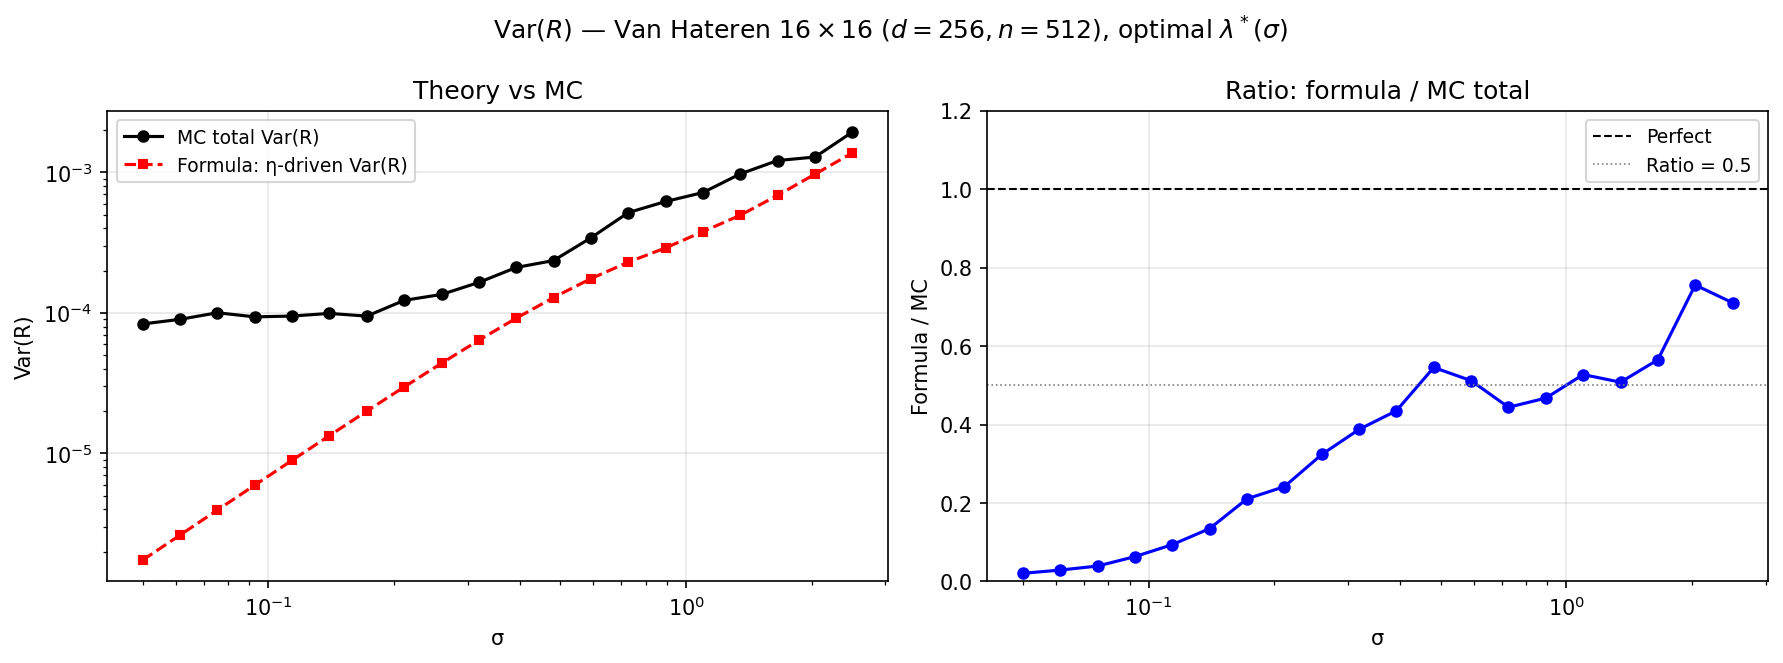
\includegraphics[width=.82\textwidth]{../figures/var_R_theory_vs_mc.png}
    \caption{Variance correction for the alignment ratio. The missing $\operatorname{Var}(R)$ term is negligible when alignment bias is large, but can dominate $\Eacc$ when $R$ is close to one.}
    \label{fig:varr}
\end{figure}

\section{Discussion}

The analysis suggests a simple lesson: evaluating a model by average prediction error can miss failures that appear when the model is used directionally. In ridge regression, the problem is already visible and exactly characterizable. The learned vector is pulled by regularization, finite-sample covariance fluctuations, and noise amplification in ways that affect average prediction and directional accentuation differently.

This setting is intentionally minimal. It does not claim that nonlinear representation accentuation reduces to ridge regression. Instead, it provides a solvable baseline for a broader phenomenon: when learned directions are used as coordinates for intervention, their geometry matters independently of scalar predictive risk. The RMT formulas identify which parts of the data spectrum and signal orientation control this geometry.

The main technical limitation is second-order fluctuation theory. Leading deterministic equivalents are enough for per-PC error, ordinary generalization, and mean alignment. They are not enough for the full accentuation second moment in regimes where $\operatorname{Var}(R)$ dominates. A complete treatment should combine deterministic equivalents with central limit theorems for quadratic functionals of anisotropic Wishart matrices.

\bibliography{accentuation_rmt_iclr2026}
\bibliographystyle{iclr2026_conference}

\appendix

\section{Detailed Derivations}
\label{app:derivations}

This appendix gives the derivations underlying the deterministic equivalents used in the main text. We keep the notation consistent with Section~\ref{eq:linear_model}: $X\in\mathbb{R}^{n\times d}$, $\widehat{\Sigma}=X^\top X/n$, $\Sigma=\sum_{k=1}^d\lambda_k \uhat_k\uhat_k^\top$, and $b_k=\uhat_k^\top\btrue$.

\subsection{Ridge Decomposition}

For the ridge estimator in equation~\eqref{eq:ridge_estimator},
\begin{align}
    \bhat
    &= (\widehat{\Sigma}+\lambda I)^{-1}\widehat{\Sigma}\btrue
    + \sigma(\widehat{\Sigma}+\lambda I)^{-1}\frac{1}{n}X^\top\epsilon ,
    \label{eq:app_bhat_decomp}\\
    \bhat-\btrue
    &= -\lambda(\widehat{\Sigma}+\lambda I)^{-1}\btrue
    + \sigma(\widehat{\Sigma}+\lambda I)^{-1}\frac{1}{n}X^\top\epsilon .
    \label{eq:app_delta_beta}
\end{align}
The first term is the shrinkage of the signal induced by ridge regularization. The second term propagates response noise through the inverse empirical covariance.

\subsection{Deterministic Equivalent and the Effective Ridge Parameter}

In the proportional limit $d/n\to\gamma$, the ridge resolvent of $\widehat{\Sigma}$ is approximated by a deterministic resolvent of $\Sigma$ with an effective regularization parameter $\kappa=\kappa(\lambda)$ satisfying
\begin{equation}
    \kappa-\lambda
    =
    \gamma\kappa\frac{1}{d}\sum_{j=1}^{d}\frac{\lambda_j}{\kappa+\lambda_j}.
    \label{eq:app_kappa_fixed_point}
\end{equation}
The derivative of $\kappa$ with respect to $\lambda$ determines the finite-sample noise factor. Rewriting equation~\eqref{eq:app_kappa_fixed_point} as
\begin{equation}
    \lambda =
    \kappa\left[
    1-\gamma\frac{1}{d}\sum_{j=1}^{d}\frac{\lambda_j}{\kappa+\lambda_j}
    \right],
\end{equation}
we obtain
\begin{align}
    \frac{d\lambda}{d\kappa}
    &=
    1-\gamma\frac{1}{d}\sum_{j=1}^{d}\frac{\lambda_j}{\kappa+\lambda_j}
    +\gamma\frac{\kappa}{d}\sum_{j=1}^{d}\frac{\lambda_j}{(\kappa+\lambda_j)^2} \\
    &=
    1-\gamma\frac{1}{d}\sum_{j=1}^{d}\frac{\lambda_j^2}{(\kappa+\lambda_j)^2}.
\end{align}
With the unnormalized degrees of freedom
\begin{equation}
    \df(\kappa)=\sum_{j=1}^{d}\frac{\lambda_j^2}{(\lambda_j+\kappa)^2},
\end{equation}
and $\gamma=d/n$, this gives
\begin{equation}
    \frac{d\lambda}{d\kappa}=1-\frac{\df(\kappa)}{n},
    \qquad
    \frac{d\kappa}{d\lambda}=\frac{n}{n-\df(\kappa)}.
    \label{eq:app_dkappa}
\end{equation}

\subsection{Per-Eigenmode Coefficient Error}

Projecting equation~\eqref{eq:app_delta_beta} onto $\uhat_k$ and squaring gives three terms: signal bias, noise variance, and a signal-noise cross term. The cross term vanishes after averaging over the response noise. Thus
\begin{align}
    \mathbb{E}\left[(\uhat_k^\top(\bhat-\btrue))^2\right]
    &=
    \lambda^2
    \mathbb{E}\left[
    {\btrue}^{\top}(\widehat{\Sigma}+\lambda I)^{-1}
    \uhat_k\uhat_k^\top
    (\widehat{\Sigma}+\lambda I)^{-1}\btrue
    \right]
    \nonumber\\
    &\quad+
    \frac{\sigma^2}{n}
    \mathbb{E}\left[
    \operatorname{Tr}\left(
    (\widehat{\Sigma}+\lambda I)^{-1}
    \uhat_k\uhat_k^\top
    (\widehat{\Sigma}+\lambda I)^{-1}
    \widehat{\Sigma}
    \right)\right].
    \label{eq:app_perpc_start}
\end{align}

For the noise term, use
\begin{equation}
    (\widehat{\Sigma}+\lambda I)^{-1}\widehat{\Sigma}
    (\widehat{\Sigma}+\lambda I)^{-1}
    =
    \frac{d}{d\lambda}\left[\lambda(\widehat{\Sigma}+\lambda I)^{-1}\right].
\end{equation}
The deterministic equivalent gives
\begin{equation}
    \mathbb{E}\left[
    \uhat_k^\top
    (\widehat{\Sigma}+\lambda I)^{-1}\widehat{\Sigma}
    (\widehat{\Sigma}+\lambda I)^{-1}
    \uhat_k
    \right]
    \asymp
    \frac{d\kappa}{d\lambda}
    \frac{\lambda_k}{(\lambda_k+\kappa)^2}.
\end{equation}
Using equation~\eqref{eq:app_dkappa}, the noise contribution becomes
\begin{equation}
    \frac{\sigma^2}{n-\df(\kappa)}
    \frac{\lambda_k}{(\lambda_k+\kappa)^2}.
    \label{eq:app_noise_term}
\end{equation}

For the signal term, we use the two-resolvent deterministic equivalent. For deterministic matrices $A,B$ with bounded rank or bounded trace norm in the population eigenbasis,
\begin{align}
    &\operatorname{Tr}\left[
    A(\widehat{\Sigma}+\lambda I)^{-1}
    B(\widehat{\Sigma}+\lambda I)^{-1}
    \right]
    \nonumber\\
    &\quad\asymp
    \frac{\kappa^2}{\lambda^2}
    \operatorname{Tr}\left[
    A(\Sigma+\kappa I)^{-1}
    B(\Sigma+\kappa I)^{-1}
    \right]
    \nonumber\\
    &\qquad+
    \frac{\kappa^2}{\lambda^2}
    \frac{
    \operatorname{Tr}\left[
    A(\Sigma+\kappa I)^{-2}\Sigma
    \right]
    \operatorname{Tr}\left[
    B(\Sigma+\kappa I)^{-2}\Sigma
    \right]}
    {n-\df(\kappa)} .
    \label{eq:app_two_resolvent}
\end{align}
Taking $A=\btrue{\btrue}^{\top}$ and $B=\uhat_k\uhat_k^\top$ yields
\begin{align}
    &\lambda^2
    \mathbb{E}\left[
    {\btrue}^{\top}(\widehat{\Sigma}+\lambda I)^{-1}
    \uhat_k\uhat_k^\top
    (\widehat{\Sigma}+\lambda I)^{-1}\btrue
    \right]
    \nonumber\\
    &\quad\asymp
    \frac{\kappa^2}{(\lambda_k+\kappa)^2}b_k^2
    +
    \frac{\kappa^2}{n-\df(\kappa)}
    \frac{\lambda_k}{(\lambda_k+\kappa)^2}
    \sum_{j=1}^{d}
    \frac{\lambda_j b_j^2}{(\lambda_j+\kappa)^2}.
    \label{eq:app_signal_term}
\end{align}
Defining
\begin{equation}
    C_{\mathrm{sig}}(\kappa)=
    \sum_{j=1}^{d}
    \frac{\lambda_j b_j^2}{(\lambda_j+\kappa)^2},
\end{equation}
and combining equations~\eqref{eq:app_noise_term} and~\eqref{eq:app_signal_term} gives the main-text formula:
\begin{align}
    \mathbb{E}\left[(\uhat_k^\top(\bhat-\btrue))^2\right]
    &\asymp
    \frac{\kappa^2}{(\lambda_k+\kappa)^2}b_k^2
    +
    \frac{1}{n-\df(\kappa)}
    \frac{\lambda_k\kappa^2}{(\lambda_k+\kappa)^2}
    C_{\mathrm{sig}}(\kappa)
    \nonumber\\
    &\quad+
    \frac{\sigma^2}{n-\df(\kappa)}
    \frac{\lambda_k}{(\lambda_k+\kappa)^2}.
    \label{eq:app_perpc_final}
\end{align}

\subsection{Generalization Error}

For a fresh test input $\x\sim\mathcal{N}(0,\Sigma)$,
\begin{align}
    E_{\mathrm{gen}}
    &=
    \mathbb{E}\left[
    ((\bhat-\btrue)^\top\x)^2
    \right] \\
    &=
    \mathbb{E}\left[
    (\bhat-\btrue)^\top\Sigma(\bhat-\btrue)
    \right] \\
    &=
    \sum_{k=1}^{d}
    \lambda_k
    \mathbb{E}\left[
    (\uhat_k^\top(\bhat-\btrue))^2
    \right].
    \label{eq:app_gen}
\end{align}
Thus average prediction error weights coefficient error along each population PC by the natural-image variance $\lambda_k$.

\subsection{Accentuation Error and Alignment Ratio}

Accentuation uses the learned direction as a control path. Consider centered accentuation samples $\x=\alpha\bhat$, with $\mathbb{E}\alpha=0$. We choose the scale so that the model-predicted variance along the accentuation path matches the natural response variance:
\begin{align}
    \operatorname{Var}(\bhat^\top(\alpha\bhat))
    &=
    (\bhat^\top\bhat)^2\operatorname{Var}(\alpha)
    =
    {\btrue}^{\top}\Sigma\btrue,\\
    \operatorname{Var}(\alpha)
    &=
    \frac{{\btrue}^{\top}\Sigma\btrue}{(\bhat^\top\bhat)^2}.
\end{align}
The accentuation error against the true response is then
\begin{align}
    \Eacc
    &=
    \mathbb{E}_{X,\epsilon,\alpha}
    \left[
    \left(\alpha\bhat^\top(\bhat-\btrue)\right)^2
    \right] \\
    &=
    {\btrue}^{\top}\Sigma\btrue\cdot
    \mathbb{E}_{X,\epsilon}
    \left[
    \frac{(\bhat^\top\bhat-\bhat^\top\btrue)^2}
    {(\bhat^\top\bhat)^2}
    \right] \\
    &=
    {\btrue}^{\top}\Sigma\btrue\cdot
    \mathbb{E}_{X,\epsilon}
    \left[
    \left(1-
    \frac{\bhat^\top\btrue}{\bhat^\top\bhat}
    \right)^2
    \right].
    \label{eq:app_acc_exact}
\end{align}
This motivates the alignment ratio
\begin{equation}
    R=\frac{\bhat^\top\btrue}{\bhat^\top\bhat}.
\end{equation}

\subsection{Deterministic Equivalent for Mean Alignment}

The numerator concentrates around
\begin{align}
    N_{\det}
    &=
    \mathbb{E}[\bhat^\top\btrue]
    \asymp
    {\btrue}^{\top}(\Sigma+\kappa I)^{-1}\Sigma\btrue \\
    &=
    \sum_{k=1}^{d}
    \frac{\lambda_k}{\lambda_k+\kappa}b_k^2.
    \label{eq:app_Ndet}
\end{align}
The denominator must be computed as $\mathbb{E}[\bhat^\top\bhat]$, not as the squared deterministic mean of $\bhat$. Using equation~\eqref{eq:app_bhat_decomp} and the per-PC second moment,
\begin{align}
    D_{\det}
    &=
    \mathbb{E}[\bhat^\top\bhat]\\
    &\asymp
    \sum_{k=1}^{d}
    \left(\frac{\lambda_k}{\lambda_k+\kappa}\right)^2 b_k^2
    +
    \frac{\kappa^2 C_{\mathrm{sig}}(\kappa)+\sigma^2}{n-\df(\kappa)}
    \sum_{k=1}^{d}
    \frac{\lambda_k}{(\lambda_k+\kappa)^2}.
    \label{eq:app_Ddet}
\end{align}
The second term in equation~\eqref{eq:app_Ddet} is crucial: it contains both finite-sample signal variance and the corrected effective-sample-size denominator for the noise term. The leading deterministic alignment is
\begin{equation}
    R_{\det}=\frac{N_{\det}}{D_{\det}},
    \qquad
    \Eacc^{(0)}
    =
    {\btrue}^{\top}\Sigma\btrue(1-R_{\det})^2.
    \label{eq:app_Rdet}
\end{equation}

\subsection{Second-Order Correction: Variance of the Alignment Ratio}

The approximation in equation~\eqref{eq:app_Rdet} captures the squared bias term in
\begin{equation}
    \mathbb{E}[(1-R)^2]=(1-\mathbb{E}R)^2+\operatorname{Var}(R),
\end{equation}
but omits $\operatorname{Var}(R)$. When $R\approx 1$, this variance term can dominate the full accentuation error.

Let $N=\bhat^\top\btrue$, $D=\bhat^\top\bhat$, and $R_{\det}=N_{\det}/D_{\det}$. A delta-method expansion gives
\begin{equation}
    R-R_{\det}
    \approx
    \frac{(N-N_{\det})-R_{\det}(D-D_{\det})}{D_{\det}}
    =
    \frac{\delta Q}{D_{\det}},
\end{equation}
where $Q=N-R_{\det}D=\bhat^\top(\btrue-R_{\det}\bhat)$. Thus
\begin{equation}
    \operatorname{Var}(R)
    \asymp
    \frac{\operatorname{Var}(Q)}{D_{\det}^2}.
    \label{eq:app_varR_Q}
\end{equation}

Decompose $\bhat=g+h$, with
\begin{align}
    g &\asymp (\Sigma+\kappa I)^{-1}\Sigma\btrue,\\
    h &\sim
    \mathcal{N}\left(0,\frac{\sigma^2}{n}H\right),
    \qquad
    H=(\Sigma+\kappa I)^{-1}\Sigma(\Sigma+\kappa I)^{-1}.
\end{align}
Keeping the noise-driven fluctuations and centering the quadratic form,
\begin{equation}
    Q
    =
    h^\top(\btrue-2R_{\det}g)
    -
    R_{\det}\left(h^\top h-\mathbb{E}[h^\top h]\right).
\end{equation}
The first term is odd in $h$ and the second is even, so they are uncorrelated. Therefore,
\begin{align}
    \operatorname{Var}(Q)
    &=
    \frac{\sigma^2}{n}
    (\btrue-2R_{\det}g)^\top H(\btrue-2R_{\det}g)
    +
    2R_{\det}^2
    \left(\frac{\sigma^2}{n}\right)^2
    \operatorname{Tr}(H^2).
\end{align}
In the eigenbasis of $\Sigma$, this becomes
\begin{align}
    \operatorname{Var}(R)
    &\asymp
    \frac{1}{D_{\det}^2}
    \left[
    \frac{\sigma^2}{n}
    \sum_{k=1}^{d}
    \frac{\lambda_k b_k^2}{(\lambda_k+\kappa)^2}
    \left(1-\frac{2R_{\det}\lambda_k}{\lambda_k+\kappa}\right)^2
    +
    \frac{2R_{\det}^2\sigma^4}{n^2}
    \sum_{k=1}^{d}
    \frac{\lambda_k^2}{(\lambda_k+\kappa)^4}
    \right].
    \label{eq:app_varR_final}
\end{align}
The full second-order accentuation approximation is
\begin{equation}
    \mathbb{E}[\Eacc]
    \asymp
    {\btrue}^{\top}\Sigma\btrue
    \left[
    (1-R_{\det})^2+\operatorname{Var}(R)
    \right].
    \label{eq:app_acc_full}
\end{equation}
Equation~\eqref{eq:app_varR_final} captures the response-noise contribution to alignment variance. A complete finite-$n$ theory should also include random-design fluctuations of $\widehat{\Sigma}$, which empirically dominate at very low response noise and require a higher-order CLT for anisotropic Wishart quadratic forms.

\subsection{Why Low-Variance Modes Are Dangerous for Control}

For ordinary least squares, the population coefficient along PC $k$ can be written heuristically as
\begin{equation}
    w_{\mathrm{OLS},k}
    =
    \sigma_y\frac{1}{\sqrt{\lambda_k}}
    \operatorname{corr}(\uhat_k^\top X,y).
\end{equation}
For ridge regression,
\begin{equation}
    w_{\mathrm{ridge},k}
    =
    \sigma_y
    \frac{\sqrt{\lambda_k}}{\lambda_k+\lambda}
    \operatorname{corr}(\uhat_k^\top X,y).
\end{equation}
OLS therefore has explicit $1/\sqrt{\lambda_k}$ amplification in low-variance directions, while ridge suppresses the most extreme blow-up but still amplifies modes near $\lambda_k\approx\lambda$ or, in the finite-sample deterministic equivalent, near $\lambda_k\approx\kappa$. This is the linear mechanism behind high-frequency, off-manifold feature accentuations: low-variance directions barely affect prediction on natural images but can dominate the model gradient used for control.


\section{Reproducibility Statement}

The theory assumptions and deterministic equivalents are stated in the main text, with detailed derivations in Appendix~\ref{app:derivations}. The accompanying validation repository contains the core RMT library, CPU and GPU Monte Carlo scripts, notebooks recreating the figures, and saved outputs for the experiments shown here. The experiments use synthetic Gaussian covariates with specified spectra and empirical natural-image covariance spectra; all random quantities are generated by the scripts.

\section{Ethics Statement}

This work is theoretical and uses synthetic simulations and natural-image covariance spectra for validation. It does not introduce a deployed model, collect human-subject data, or release a dataset with personal information. The main risk is interpretive: directional analyses can be misleading if treated as causal without appropriate assumptions. The paper therefore emphasizes the limits of average test error and the assumptions required for the proposed metric.

\end{document}
